\section{Chi tiết dự án}

\indent Các thiết bị được sử dụng trong dự án này bào gồm: 
\begin{itemize}
    \item 1 flex sensor 2.2 inch
    \item 4 flex sensor 4.5 inch
    \item 1 mạch arduino nano
\end{itemize}

\subsection{Tổng quát dự án}

\indent Dự án này tập trung vào việc thu thập và xử lý dữ liệu từ cảm biến Flex Sensor, sau đó triển khai mô hình AI để dự đoán giá trị dựa trên dữ liệu thu thập. Cấu trúc dự án bao gồm các thành phần chính sau:

\begin{figure}[H]
    \centering
    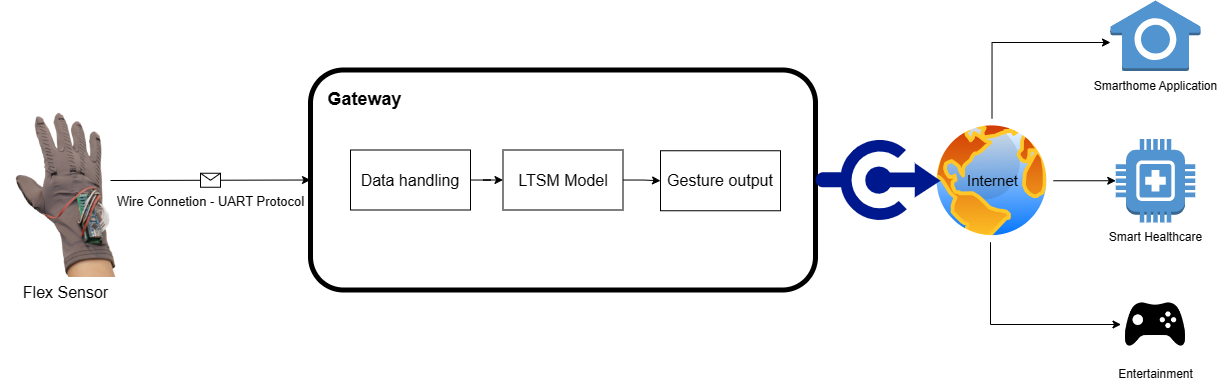
\includegraphics[scale=0.25]{Images/Theoretical basis/FlexArchitecture (1).png}
    \caption{Kiến trúc tổng quan của hệ thống}
    \label{fig:ProjectArchitecture}
\end{figure}

\begin{enumerate}[-]
    \item Kết nối cảm biến Flex Sensor, Arduino và Gateway 
    \begin{itemize}
        \item Cảm biến Flex Sensor được kết nối với Arduino qua chân đầu vào analog.
        \item Arduino chịu trách nhiệm đọc dữ liệu từ cảm biến, áp dụng bộ lọc Kalman để ổn định và truyền thông tin đến gateway qua cổng USB.
    \end{itemize}
    \item  Thu thập và chuẩn bị dữ liệu
    \begin{itemize}
        \item Máy tính hoặc gateway thực hiện quá trình thu thập dữ liệu từ Arduino bằng cách thực thi script Python.
        \item Dữ liệu thu thập được lưu vào tệp văn bản, tạo nền tảng cho việc đào tạo mô hình AI.
    \end{itemize}
    \item  Đào tạo và triển khai mô hình AI
    \begin{itemize}
        \item Mô hình AI được xây dựng, huấn luyện và triển khai trên gateway.
        \item Dữ liệu từ tệp văn bản được định dạng lại để phù hợp với cấu trúc đầu vào của mô hình LSTM.
        \item Mô hình AI dự đoán giá trị từ các cảm biến Flex Sensor dựa trên mẫu dữ liệu đã học từ quá trình huấn luyện.
    \end{itemize}
    \item Kết quả thu thập được từ mô hình sẽ được sử dụng vào các ứng dụng như nhà thông minh, thiết bị y tế thông minh, giải trí đa phương tiện,...
\end{enumerate}

\subsection{Đọc dữ liệu từ Flex Sensor}

\subsubsection{Nguyên lý}

\indent Trong phần này, chúng tôi triển khai quá trình đọc dữ liệu từ 5 cảm biến Flex Sensor sử dụng Arduino Nano và áp dụng bộ lọc Kalman để tối ưu hóa độ chính xác và ổn định của dữ liệu thu thập được. Đây là một phần quan trọng của hệ thống, giúp đảm bảo rằng dữ liệu đo lường là chính xác và có thể tin cậy.

\subsubsection{Chi tiết cách hoạt động}

\begin{enumerate}[-]
    \item Bộ lọc Kalman:
    \begin{itemize}
        \item Chúng tôi sử dụng thư viện SimpleKalmanFilter để tạo và cấu hình 5 bộ lọc Kalman (bo\_loc1 đến bo\_loc5). Các bộ lọc này đảm bảo rằng giá trị đọc từ các cảm biến được ổn định và giảm thiểu nhiễu.
    \end{itemize}
    \item  Đọc dữ liệu từ 5 Flex Sensor:
    \begin{itemize}
        \item Sử dụng hàm analogRead() để đọc giá trị analog từ 5 cảm biến Flex Sensor (A1 đến A5).
    \end{itemize}
    \item  Sử dụng bộ lọc Kalman:
    \begin{itemize}
        \item Mỗi giá trị đọc từ cảm biến Flex Sensor được truyền qua hàm updateEstimate của bộ lọc Kalman để ổn định dữ liệu và giảm nhiễu.
    \end{itemize}
    \item  Hiển thị dữ liệu và điều khiển LED:
    \begin{itemize}
        \item In giá trị đã lọc từ 5 cảm biến ra cổng Serial để theo dõi trên máy tính.
        \item Sử dụng LED kết nối với chân A0 để tạo hiệu ứng nhấp nháy. LED được điều khiển qua cổng PWM (analogWrite) để thay đổi độ sáng. LED được sử dụng để kiểm tra hệ thống có hoạt động chính xác hay không.
    \end{itemize}
    \item  Kiểm tra thời gian để in kết quả đo ra màn hình:
    \begin{itemize}
        \item Kiểm tra xem đã đủ thời gian giữa các lần in ra màn hình chưa (49ms). Điều này giúp hiển thị dữ liệu một cách đều đặn.
    \end{itemize}
    \item  Delay và lặp lại:
    \begin{itemize}
        \item Đợi 10ms trước khi lặp lại quá trình đọc dữ liệu từ cảm biến. Thời gian này cũng giúp kiểm soát tốc độ lấy mẫu và xử lý dữ liệu
    \end{itemize}
\end{enumerate}


\subsubsection{Mã nguồn}

\indent Mã nguồn được nạp vào Arduino Nano thông qua Arduino IDE

\begin{lstlisting}
#include <SimpleKalmanFilter.h>

SimpleKalmanFilter bo_loc1(2, 2, 0.1);
SimpleKalmanFilter bo_loc2(2, 2, 0.1);
SimpleKalmanFilter bo_loc3(2, 2, 0.1);
SimpleKalmanFilter bo_loc4(2, 2, 0.1);
SimpleKalmanFilter bo_loc5(2, 2, 0.1);

unsigned long previousMillis = 0;  
const long interval = 49;   
int i = 0;

void setup() {
  Serial.begin(115200);
  pinMode(A0, OUTPUT);
}

void loop() {
  unsigned long currentMillis = millis();
  
  int flex1 = analogRead(A1);
  int flex2 = analogRead(A2);
  int flex3 = analogRead(A3);
  int flex4 = analogRead(A4);
  int flex5 = analogRead(A5);

  flex1 = bo_loc1.updateEstimate(flex1);
  flex2 = bo_loc2.updateEstimate(flex2);
  flex3 = bo_loc3.updateEstimate(flex3);
  flex4 = bo_loc4.updateEstimate(flex4);
  flex5 = bo_loc5.updateEstimate(flex5);

  Serial.print(flex1);
  Serial.print("\t");
  Serial.print(flex2);
  Serial.print("\t");
  Serial.print(flex3);
  Serial.print("\t");
  Serial.print(flex4);
  Serial.print("\t");
  Serial.print(flex5);
  Serial.println();
  if (i % 2 == 0)
    analogWrite(A0, 0);
  else
    analogWrite(A0, 1023);
  i++;
  delay(10); 
}
\end{lstlisting}

\subsection{Thu thập và chuẩn bị dữ liệu}

\subsubsection{Nguyên lý}

\indent Trong phần này, chúng tôi trình bày quá trình sử dụng mã nguồn Python để thu thập và chuẩn bị dữ liệu từ cảm biến Flex Sensor. Mục đích là đọc dữ liệu từ cổng serial và lưu vào tệp văn bản, tạo nền tảng cho việc phân tích và đào tạo mô hình AI.

\subsubsection{Chi tiết cách hoạt động}

\begin{enumerate}[-]
    \item Đọc và ghi dữ liệu từ Cổng Serial:
    \begin{itemize}
        \item Sử dụng thư viện serial để thiết lập kết nối với cổng serial.
        \item Thiết lập tên cổng serial (SERIA\_PORT) và tốc độ truyền (SERIAL\_RATE) để kết nối với Arduino Nano.
        \item Sử dụng time.sleep(2) để đảm bảo thiết bị đã sẵn sàng nhận dữ liệu.
        \item Mở kết nối với cổng serial và thiết lập thời gian chờ (timeout).
    \end{itemize}
    \item  Ghi dữ liệu vào tệp văn bản:
    \begin{itemize}
        \item Mở tệp văn bản (output.txt) trong chế độ ghi ('w') để xóa nội dung cũ và chuẩn bị cho việc ghi mới.
        \item Trong vòng lặp, đọc dữ liệu từ cổng serial bằng cách sử dụng ser.readline().decode('utf-8').
        \item Hiển thị dữ liệu trên màn hình console và ghi vào tệp văn bản.
    \end{itemize}
    \item  Dừng quá trình thu thập dữ liệu:
    \begin{itemize}
        \item Sử dụng KeyboardInterrupt để dừng quá trình khi người dùng nhấn Ctrl+C.
        \item Đóng kết nối serial và thông báo khi kết thúc thu thập dữ liệu.
    \end{itemize}
\end{enumerate}

\subsubsection{Mã nguồn}

\indent Mã nguồn được chạy trên gateway

\begin{lstlisting}
import serial
import time
// this port address is for the serial tx/rx pins on the GPIO header
SERIAL_PORT = '/dev/cu.usbserial-14430'
// be sure to set this to the same rate used on the Arduino
SERIAL_RATE = 115200
OUTPUT_FILE_NAME = 'output.txt'  // Specify the output file name

def main():
    time.sleep(2)
    ser = serial.Serial(SERIAL_PORT, SERIAL_RATE,timeout=0.01)
    ser.reset_output_buffer()
    // Open the file for writing
    with open(OUTPUT_FILE_NAME, 'w') as output_file:
        print(f"Recording data to '{OUTPUT_FILE_NAME}'. Press Ctrl+C to stop.")
        
        try:
            while True:
                reading = ser.readline().decode('utf-8')
                print(reading, end='')  // Print without newlines
                // Write the reading to the file
                output_file.write(reading)
        except KeyboardInterrupt:
            pass
        finally:
            ser.close()
            print("\nSerial connection closed.")

if __name__ == "__main__":
    main()
\end{lstlisting}

\subsection{Định dạng lại dữ liệu cho mô hình LSTM}

\subsubsection{Nguyên lý}

\indent Trong phần này, chúng tôi trình bày cách sử dụng mã nguồn Python để định dạng lại dữ liệu từ cảm biến Flex Sensor. Mục tiêu là chuẩn bị dữ liệu để huấn luyện mô hình LSTM bằng cách sắp xếp lại và chia nhỏ thành các mẫu có kích thước phù hợp.

\subsubsection{Chi tiết cách hoạt động}

\begin{enumerate}[-]
    \item Xác định kích thước dữ liệu định dạng lại:
    \begin{itemize}
        \item Số cảm biến (NUM\_OF\_SENSOR) và số lần lấy mẫu (NUM\_OF\_SAMPLING) được xác định từ trước.
        \item Tính toán số cột mới sau khi định dạng lại (new\_num\_columns).
    \end{itemize}
    \item  Xác định đường dẫn và tên tệp
    \begin{itemize}
        \item Đường dẫn và tên tệp được xác định chính xác cho cả dữ liệu gốc và dữ liệu mới được định dạng lại.
    \end{itemize}
    \item  Load dữ liệu gốc:
    \begin{itemize}
        \item Dữ liệu được tải từ tệp văn bản gốc thông qua np.loadtxt.
    \end{itemize}
    \item  Định dạng lại dữ liệu:
    \begin{itemize}
        \item Một mảng mới được tạo ra với số cột mới.
        \item Hàm reformat\_data chịu trách nhiệm sắp xếp và chia nhỏ dữ liệu theo định dạng mong muốn.
        \item Dữ liệu sẽ được chia thành các cột tương ứng với mỗi lần lấy mẫu từ mỗi cảm biến.
    \end{itemize}
    \item  Hiển thị và lưu trữ kết quả
    \begin{itemize}
        \item Dữ liệu sau khi được định dạng lại sẽ hiển thị ra màn hình và được lưu vào tệp văn bản mới.
    \end{itemize}
\end{enumerate}

\subsubsection{Mã nguồn}

\indent Mã nguồn được chạy trên gateway

\begin{lstlisting}
import numpy as np
from numpy import array

// Define new shape of formated data
NUM_OF_SENSOR = 5
NUM_OF_SAMPLING = 120

new_num_columns = NUM_OF_SENSOR * NUM_OF_SAMPLING

// Replace 'path/to/your/original_file.txt' and 'path/to/your/new_file.txt'
// with the actual paths for your original and new text files
original_file_path = 'datatrain/label1.txt'
new_file_path = 'datatrain/label1_reshape.txt'

// Load data from the original text file
original_data = np.loadtxt(original_file_path)

def add_overlap_to_rows(arr):
    new_rows = [arr[0]]
    
    for i in range(1, len(arr)):
        overlap = arr[i][:len(arr[i]) // 2]
        new_row = np.concatenate((new_rows[-1][len(overlap):], overlap))
        new_rows.append(new_row)

    return np.array(new_rows)

print("Original data:")
print(original_data)
print("Shape of the original data:", original_data.shape)

formated_data = np.zeros(shape=(1, new_num_columns))

def reformat_data(arr):
    temp_rows = [0 for i in range(new_num_columns)] 
    idx = 0
    global formated_data
    for i in range(0, len(arr)):
        if(idx == 120) :
            idx = 0
            formated_data = np.append(formated_data, [temp_rows], axis=0)
        temp_rows[idx] = arr[i][0]
        temp_rows[idx + 120] = arr[i][1]
        temp_rows[idx + 240] = arr[i][2]
        temp_rows[idx + 360] = arr[i][3]
        temp_rows[idx + 480] = arr[i][4]
        idx = idx + 1
    formated_data = np.delete(formated_data, (0), axis=0)

reformat_data(original_data)

print("\nReshaped data with 120 * 5 columns:")
print(formated_data)

// Save the reshaped data to a new text file
np.savetxt(new_file_path, formated_data, fmt='%.f', delimiter=' ')

print(f"\nReshaped data saved to {new_file_path}")
\end{lstlisting}

\subsection{Mô hình LSTM}

\subsubsection{Cơ sở lý thuyết}


\subsubsubsection{Ý tưởng đằng sau LSTM}

\begin{figure}[H]
    \centering
    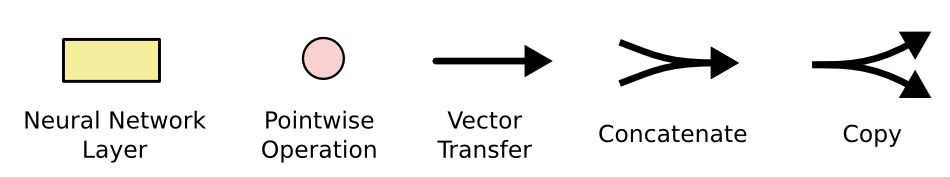
\includegraphics[width=14cm]{Images/Architecture/lstm1.png}
\caption{Diễn giải các kí hiệu trong đồ thị}
\end{figure}

\indent 

\begin{itemize}
    \item Ý tưởng chính của LSTM là thành phần ô trạng thái (cell state) được thể hiện qua đường chạy ngang qua đỉnh đồ thị như hình vẽ bên dưới:
    \begin{figure}[H]
        \centering
        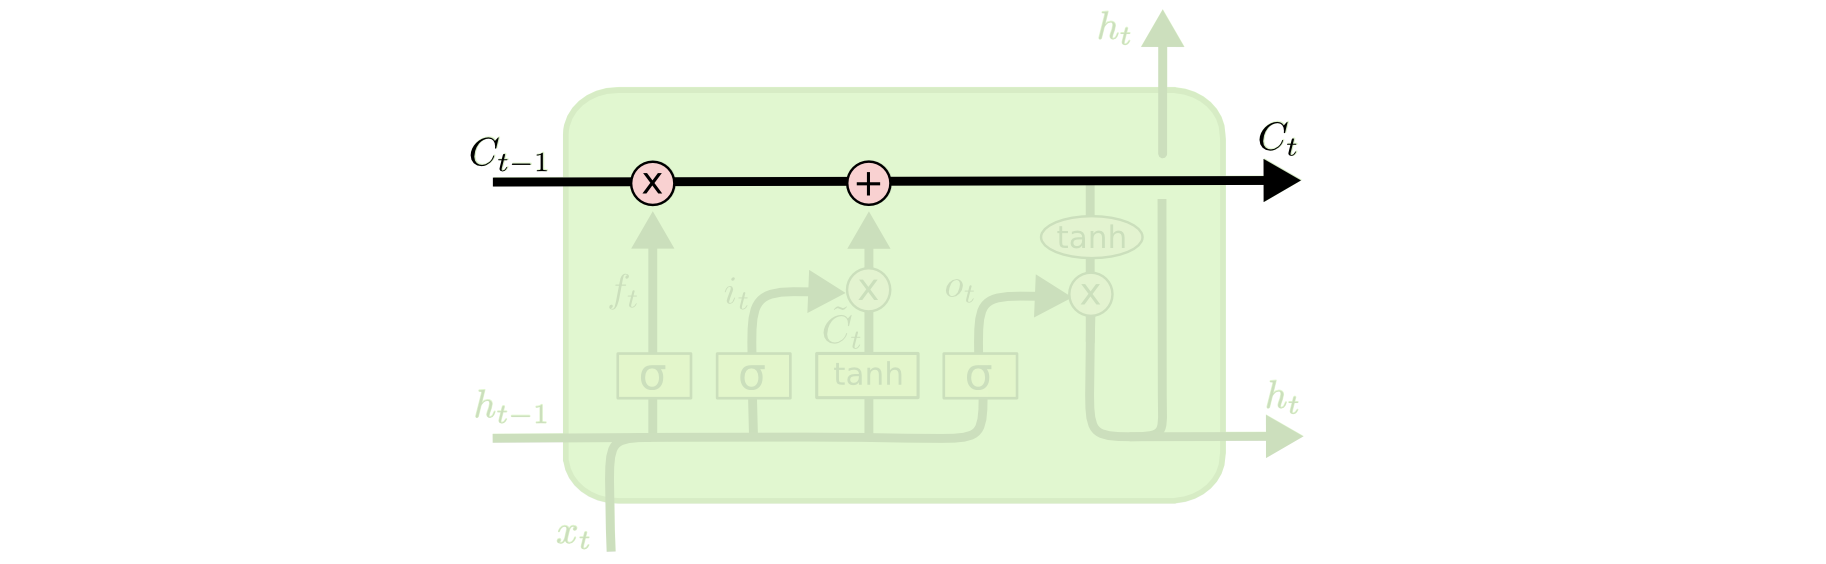
\includegraphics[width=14cm]{Images/Architecture/LSTM3-C-line.png}
    \caption{Đường đi của ô trạng thái (cell state) trong mạng LSTM}
    \end{figure}
    \item Ô trạng thái là một dạng băng chuyền chạy thẳng xuyên suốt toàn bộ chuỗi với chỉ một vài tương tác tuyến tính nhỏ giúp cho thông tin có thể truyền dọc theo đồ thị mạng nơ-ron ổn định.
    \item LSTM có khả năng xóa và thêm thông tin vào ô trạng thái và điều chỉnh các luồng thông tin này thông qua các cấu trúc gọi là cổng.
    \item Cổng là cơ chế đặc biệt để điều chỉnh luồng thông tin đi qua. Chúng được tổng hợp bởi một tầng ẩn của hàm activation sigmoid và với một toán tử nhân như đồ thị.
    \begin{figure}[H]
        \centering
        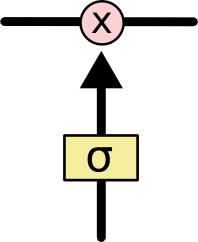
\includegraphics[width=3cm]{Images/Architecture/LSTM3-gate.png}
    \caption{Một cổng của hàm sigmoid trong LSTM}
    \end{figure}
    \item Hàm sigmoid sẽ cho đầu ra là một giá trị xác xuất nằm trong khoảng từ 0 đến 1, thể hiện rằng có bao nhiêu phần thông tin sẽ đi qua cổng. Giá trị bằng 0 ngụ ý rằng không cho phép thông tin nào đi qua, giá trị bằng 1 sẽ cho toàn bộ thông tin đi qua.
    \item Một mạng LSTM sẽ có 3 cổng có kiến trúc dạng này để bảo vệ và kiểm soát các ô trạng thái.
\end{itemize}

\subsubsubsection{Thứ tự các bước của LSTM}

\indent Bước đầu tiên trong LSTM sẽ quyết định xem thông tin nào chúng ta sẽ cho phép đi qua ô trạng thái (cell state). Nó được kiểm soát bởi hàm sigmoid trong một tầng gọi là tầng quên (forget gate layer). Đầu tiên nó nhận đầu vào là 2 giá trị \( h_{t-1} \)
 và \( x_{t} \)
 và trả về một giá trị nằm trong khoảng 0 và 1 cho mỗi giá trị của ô trạng thái \( \text{C}_{t-1} \)
. Nếu giá trị bằng 1 thể hiện ‘giữ toàn bộ thông tin’ và bằng 0 thể hiện ‘bỏ qua toàn bộ chúng’.

\indent Trở lại ví dụ về ngôn ngữ, chúng ta đang cố gắng dự báo từ tiếp theo dựa trên toàn bộ những từ trước đó. Trong những bài toán như vậy, ô trạng thái có thể bao gồm loại của chủ ngữ hiện tại, để cho đại từ ở câu tiếp theo được sử dụng chính xác. Chẳng hạn như chúng ta đang mô tả về một người bạn là con trai thì các đại từ nhân xưng ở tiếp theo phải là anh, thằng, hắn thay vì cô, con ấy. Tuy nhiên chủ ngữ không phải khi nào cũng cố định. Khi chúng ta nhìn thấy một chủ ngữ mới, chúng ta muốn quên đi loại của một chủ ngữ cũ. Do đó tầng quên cho phép cập nhật thông tin mới và lưu giữ giá trị của nó khi có thay đổi theo thời gian.

\begin{figure}[H]
    \centering
    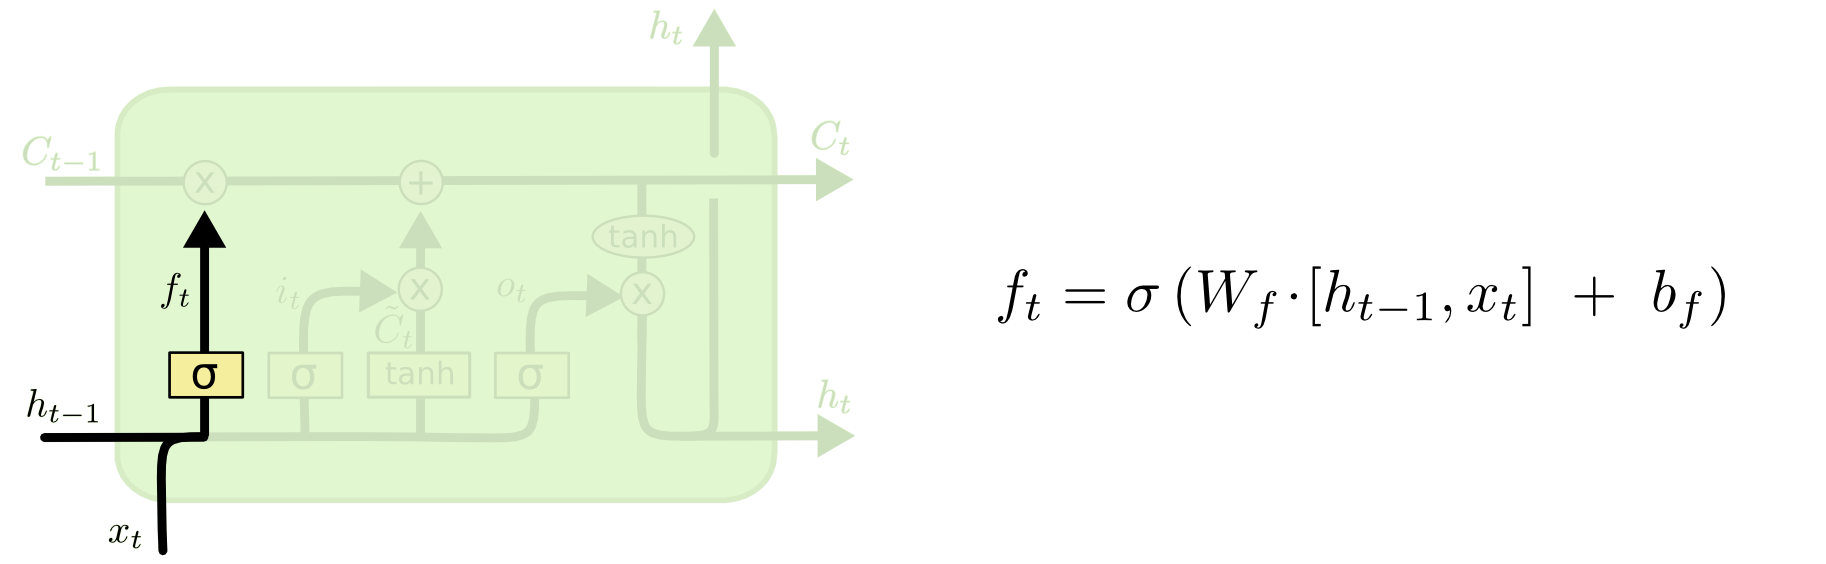
\includegraphics[width=14cm]{Images/Architecture/LSTM3-focus-f.png}
\caption{Tầng cổng quên (forget gate layer)}
\end{figure}

\indent Bước tiếp theo chúng ta sẽ quyết định loại thông tin nào sẽ được lưu trữ trong ô trạng thái. Bước này bao gồm 2 phần. Phần đầu tiên là một tầng ẩn của hàm sigmoid được gọi là tầng cổng vào (input gate layer) quyết định giá trị bao nhiêu sẽ được cập nhật. Tiếp theo, tầng ẩn hàm tanh sẽ tạo ra một véc tơ của một giá trị trạng thái mới 
 mà có thể được thêm vào trạng thái. Tiếp theo kết hợp kết quả của 2 tầng này để tạo thành một cập nhật cho trạng thái.

 \indent Trong ví dụ của mô hình ngôn ngữ, chúng ta muốn thêm loại của một chủ ngữ mới vào ô trạng thái để thay thế phần trạng thái cũ muốn quên đi.

\begin{figure}[H]
    \centering
    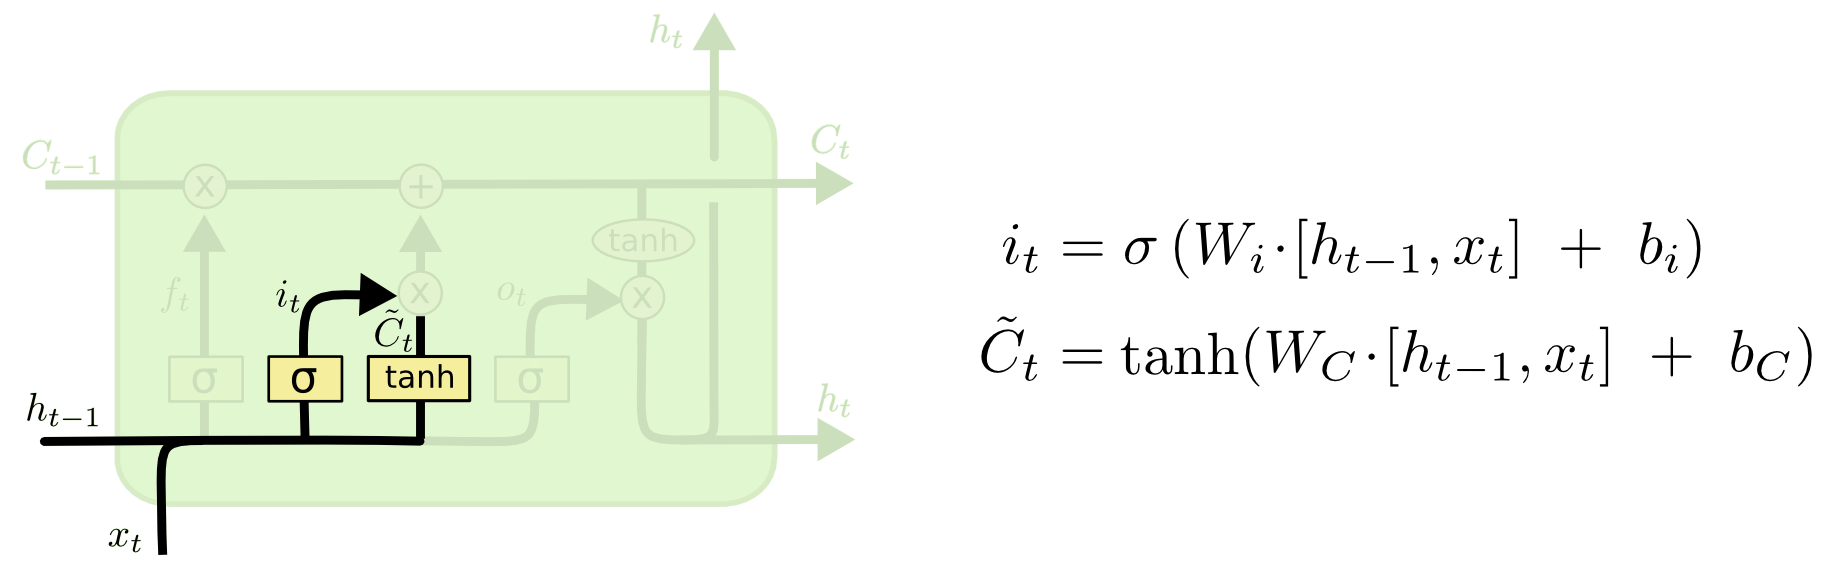
\includegraphics[width=14cm]{Images/Architecture/LSTM3-focus-i.png}
\caption{ Cập nhật giá trị cho ô trạng thái bằng cách kết hợp 2 kết quả từ tầng cổng vào và tẩng ẩn hàm tanh}
\end{figure}

\indent Đây là thời điểm để cập nhật một ô trạng thái cũ \( \text{C}_{t-1} \)
 sang một trạng thái mới \( \text{C}_{t} \)
. Những bước trước đó đã quyết định làm cái gì, và tại bước này chỉ cần thực hiện nó.

\indent Chúng ta nhân trạng thái cũ với \( f_{t} \)
 tương ứng với việc quên những thứ quyết định được phép quên sớm. Phần tử đề cử \( \tilde{\text{C}}_{t-1} \)
 là một giá trị mới được tính toán tương ứng với bao nhiêu được cập nhật vào mỗi giá trị trạng thái.

 \begin{figure}[H]
    \centering
    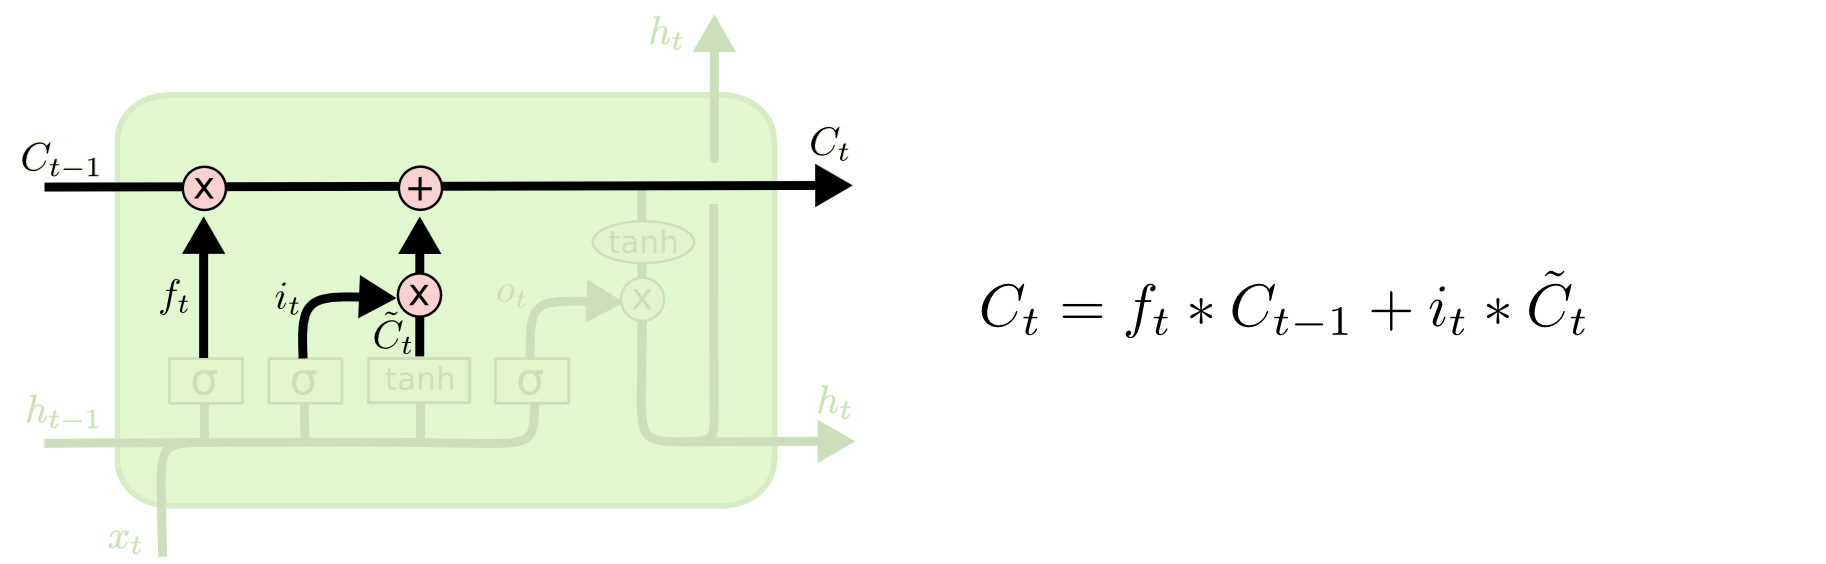
\includegraphics[width=14cm]{Images/Architecture/LSTM3-focus-C.png}
\caption{Ô trạng thái mới}
\end{figure}

\indent Cuối cùng cần quyết định xem đầu ra sẽ trả về bao nhiêu. Kết quả ở đầu ra sẽ dựa trên ô trạng thái, nhưng sẽ là một phiên bản được lọc. Đầu tiên, chúng ta chạy qua một tầng sigmoid nơi quyết định phần nào của ô trạng thái sẽ ở đầu ra. Sau đó, ô trạng thái được đưa qua hàm tanh (để chuyển giá trị về khoảng -1 và 1) và nhân nó với đầu ra của một cổng sigmoid, do đó chỉ trả ra phần mà chúng ta quyết định.

 \begin{figure}[H]
    \centering
    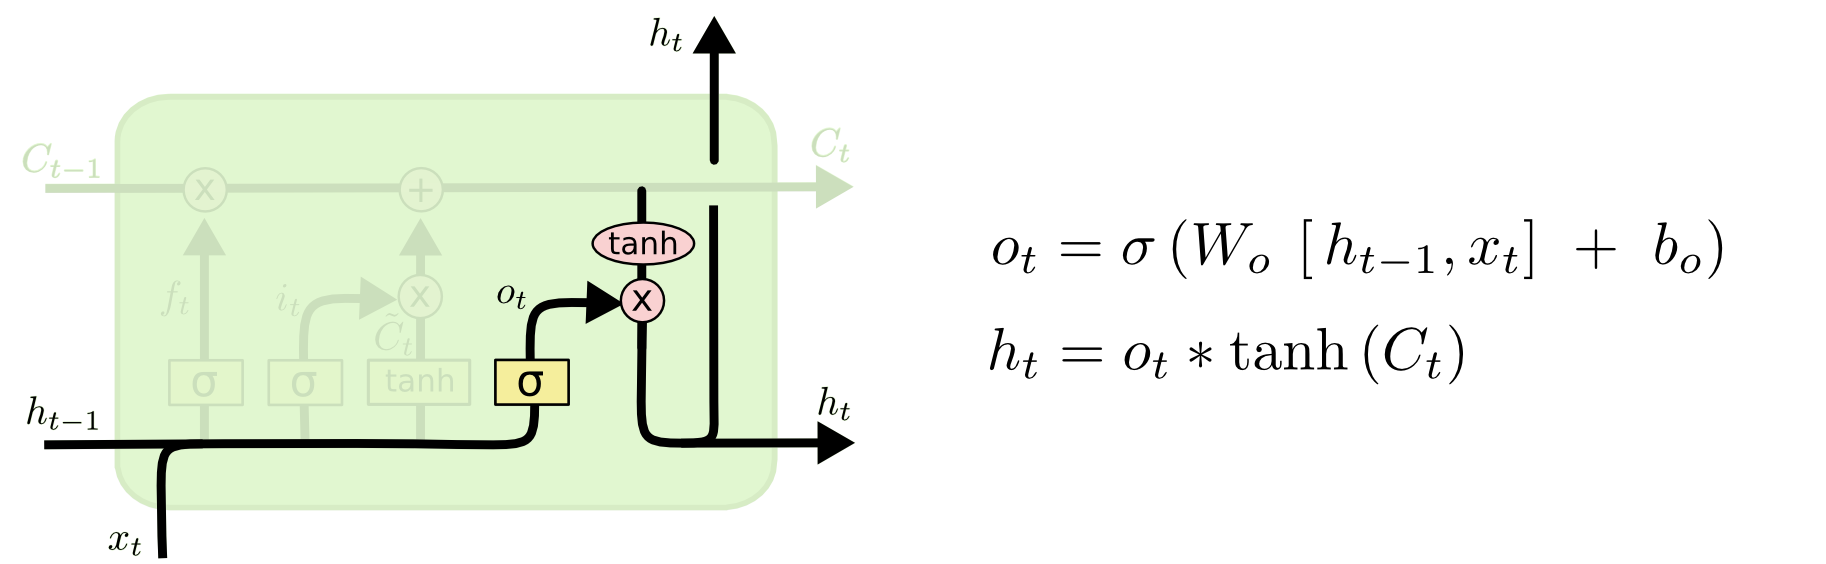
\includegraphics[width=14cm]{Images/Architecture/LSTM3-focus-o.png}
\caption{Điều chỉnh thông tin ở đầu ra thông qua hàm tanh}
\end{figure}

